\newpage
\subsection{Diagramma della Soluzione}

\begin{figure}[h]
	\includepdf[pages=-, scale=0.75]{res/DOC_OBJECT/all.pdf}
\end{figure}

\newpage

\begin{center}
	\textbf{Gui Package}
\end{center}

<<<<<<< Updated upstream
\begin{figure}[h]
	\includepdf[pages=-, scale=0.75]{res/DOC_OBJECT/gui.pdf}
\end{figure}
=======
%\begin{figure}[h]
%	\includepdf[pages=-]{res/DOC_OBJECT/gui.pdf}
%\end{figure}
>>>>>>> Stashed changes

\newpage

\begin{center}
	\textbf{Controller Package}
\end{center}

<<<<<<< Updated upstream
\begin{figure}[h]
	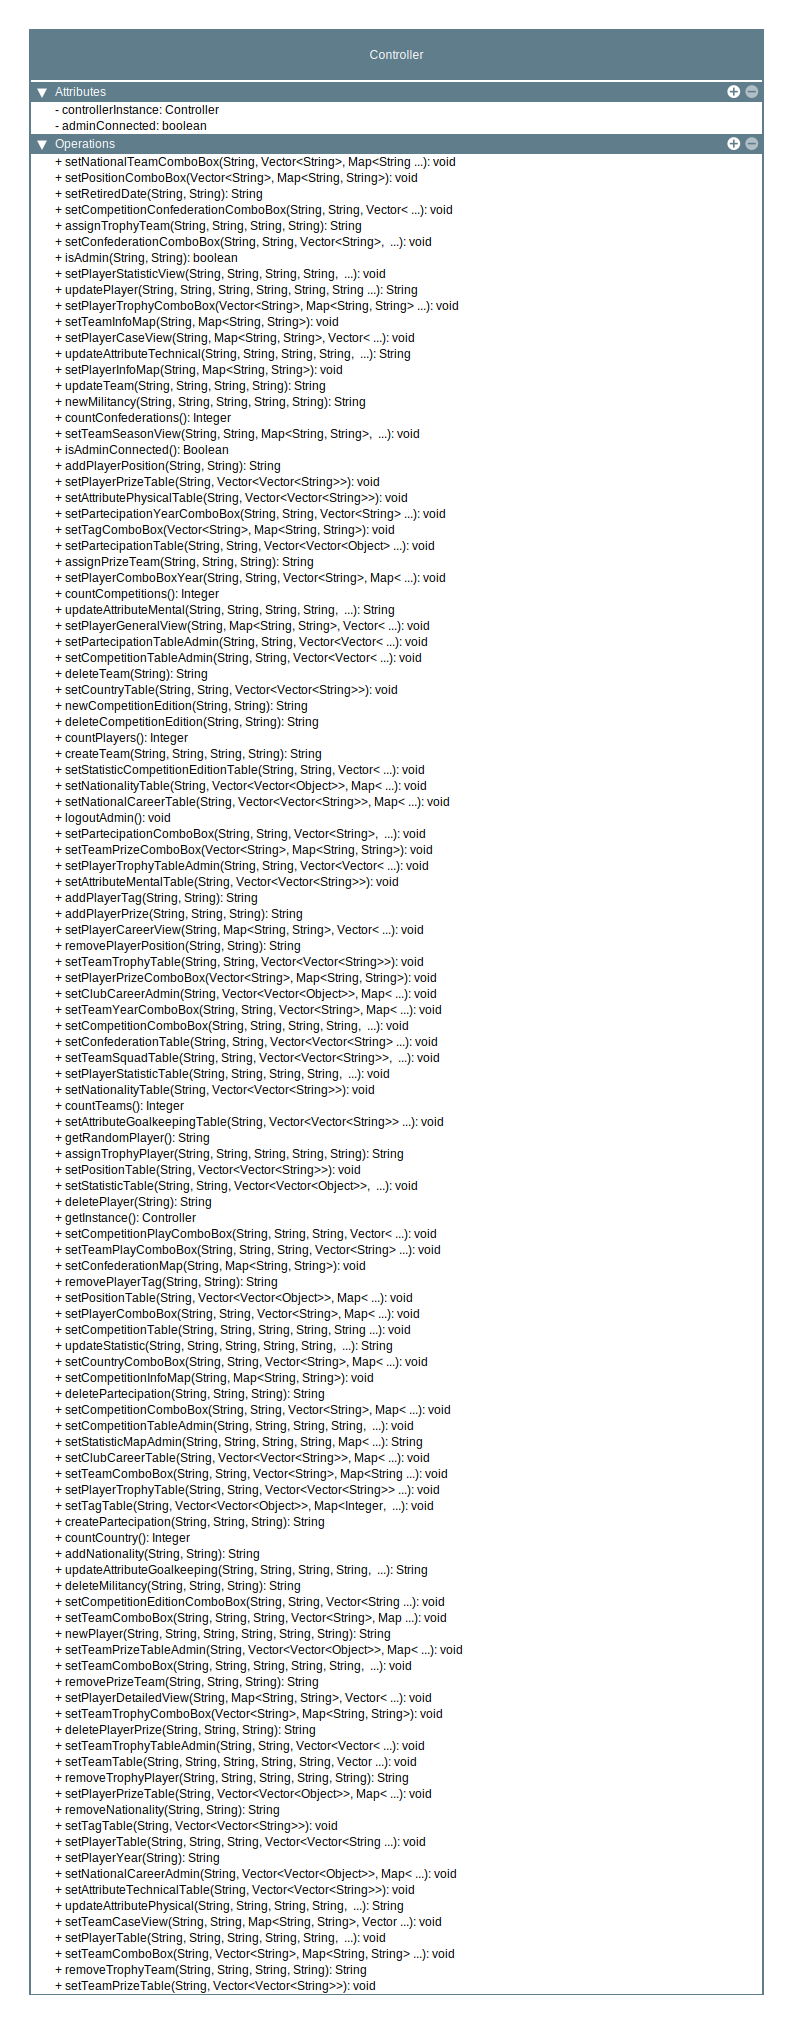
\includepdf[pages=-, scale=0.75]{res/DOC_OBJECT/controller.pdf}
\end{figure}
=======
%\begin{figure}[h]
%	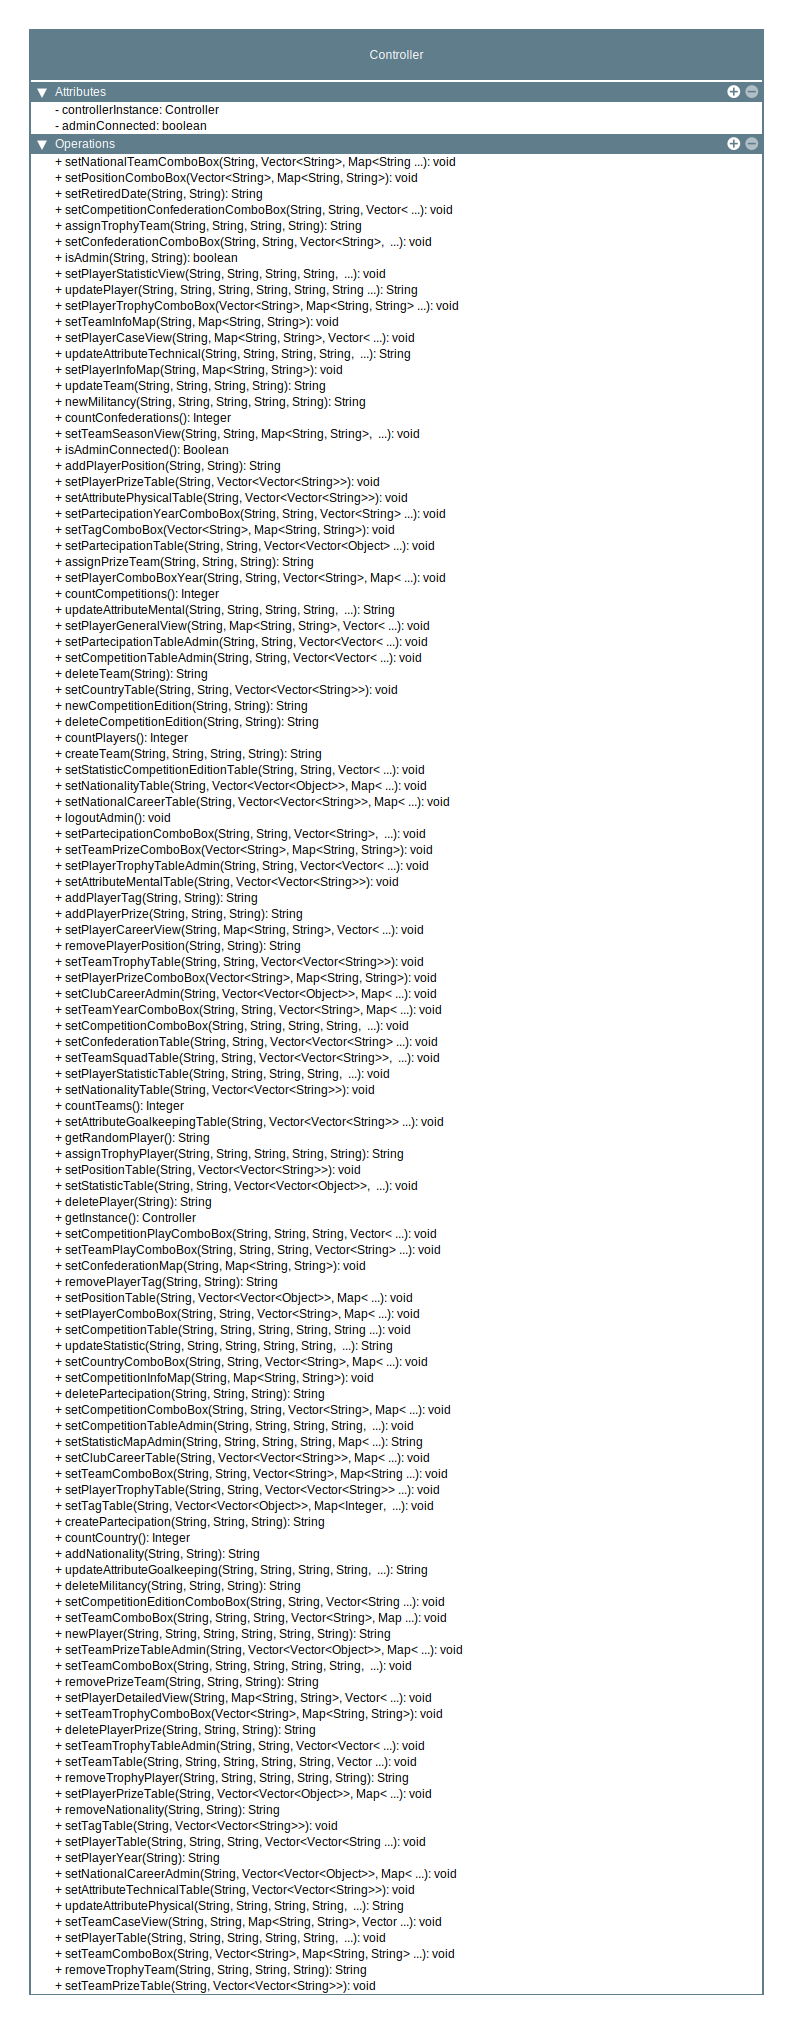
\includepdf[pages=-]{res/DOC_OBJECT/controller.pdf}
%\end{figure}
>>>>>>> Stashed changes

\newpage

\begin{center}
	\textbf{Model Package}
\end{center}

\begin{figure}[h]
<<<<<<< Updated upstream
	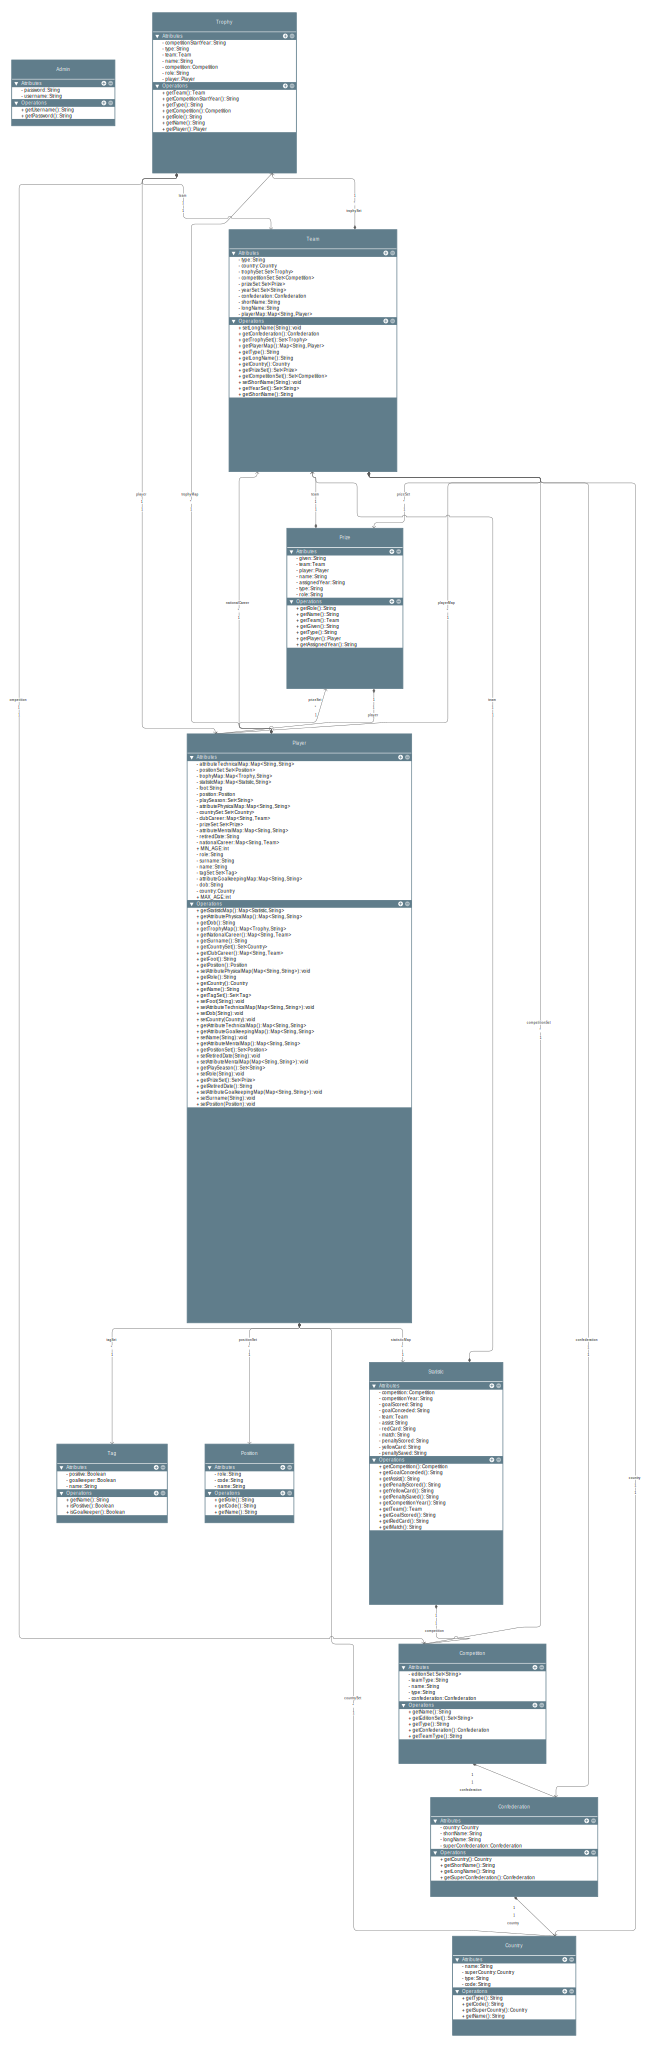
\includepdf[pages=-, scale=0.75]{res/DOC_OBJECT/model.pdf}
=======
%	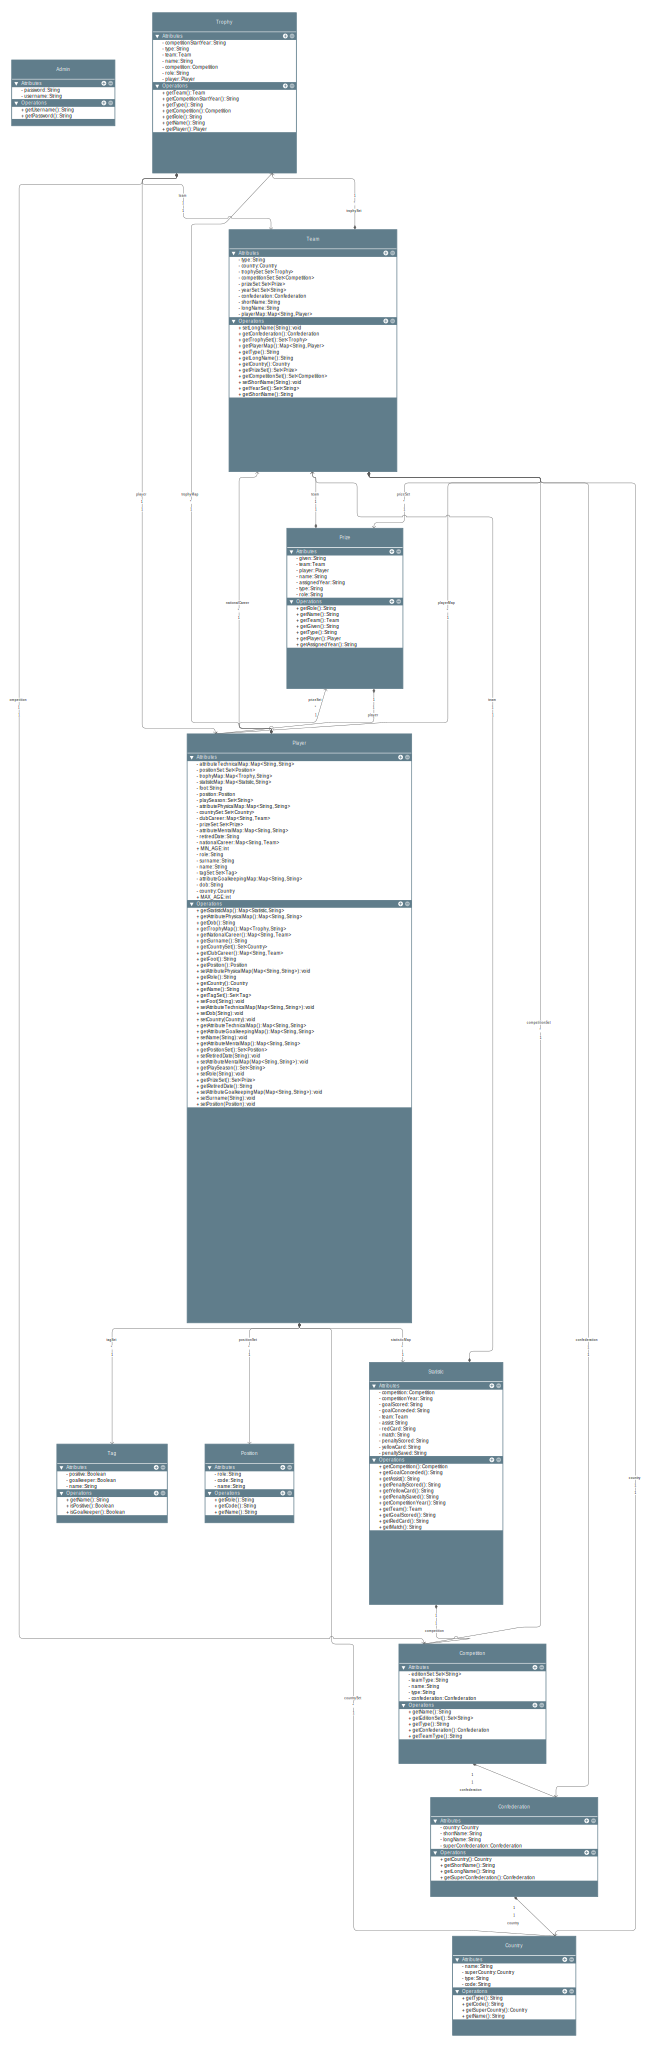
\includepdf[pages=-]{res/DOC_OBJECT/model.pdf}
>>>>>>> Stashed changes
\end{figure}

\newpage

\begin{center}
	\textbf{Dao Package}
\end{center}

\begin{figure}[h]
<<<<<<< Updated upstream
	\includepdf[pages=-, scale=0.75]{res/DOC_OBJECT/dao.pdf}
=======
%	\includepdf[pages=-]{res/DOC_OBJECT/dao.pdf}
>>>>>>> Stashed changes
\end{figure}

\newpage

\begin{center}
	\textbf{PostgreImplDao Package}
\end{center}
<<<<<<< Updated upstream

\begin{figure}[h]
	\includepdf[pages=-, scale=0.75]{res/DOC_OBJECT/PostgresImplDAO.pdf}
\end{figure}
=======
\bigskip


%\begin{figure}[h]
%	\includepdf[pages=-]{res/DOC_OBJECT/PostgreImplDAO.pdf}
%\end{figure}

\newpage

\bigskip
\begin{center}
	\textbf{ViewAll Package}
\end{center}
\bigskip

>>>>>>> Stashed changes

\newpage

\begin{center}
%	\textbf{viewOnly Package}
\end{center}

\begin{figure}[h]
	\includegraphics{res/DOC_OBJECT/onlyPackage.png}
\end{figure}






